%=========================================================================
% Example Using the Automatic LaTeX Build System
%=========================================================================
% We use hackdocumentclass because otherwise the build system will try to
% scan through IEEEtran.cls which gets it really confused.

\newcommand{\hackdocumentclass}{\documentclass}
\hackdocumentclass[journal,twoside]{IEEEtran}
\usepackage{cbxutils}

% Automatix LaTeX build system modules

\usepackage{svg}
\usepackage{py}

\begin{document}

%-------------------------------------------------------------------------
% Front Matter
%-------------------------------------------------------------------------

\title
{%
  Example Using the Automatic LaTeX Build System
}

\author
{%
  Christopher Batten,~\IEEEmembership{Member,~IEEE}%
  \thanks{C. Batten was with the Department of Electrical and Computer
    Engineering, Cornell University, Ithaca, NY, 14753 USA e-mail:
    \TT{cbatten@cornell.edu}}%
}

\markboth
{%
  Journal on Computer Systems,~Vol.~XX, No.~YY, June~YYYY
}%
{%
  Batten \MakeLowercase{\textit{et al.}}: Example of Using the Automatic
  LaTeX Build System
}

\maketitle

%-------------------------------------------------------------------------
% Body
%-------------------------------------------------------------------------

%=========================================================================
% Abstract
%=========================================================================

\begin{abstract}
  \lipsum[1]
\end{abstract}



% Putting the introduction inline here to demonstrate use of
% \IEEEPARstart

\section{Introduction}
\label{sec-intro}

\IEEEPARstart{L}{orem} Lorem ipsum dolor sit amet, consectetuer
adipiscing elit. Ut purus elit, vestibulum ut, placerat ac, adipiscing
vitae, felis. Curabitur dic- tum gravida mauris. Nam arcu libero, nonummy
eget, consectetuer id, vulputate a, magna. Donec vehicula augue eu neque.
Pellen- tesque habitant morbi tristique senectus et netus et malesuada
fames ac turpis egestas. Mauris ut leo. Cras viverra metus rhoncus sem.
Nulla et lectus vestibulum urna fringilla ultrices. Phasellus eu tellus
sit amet tortor gravida placerat. Integer sapien est, iaculis in, pretium
quis, viverra ac, nunc. Praesent eget sem vel leo ultri- ces bibendum.
Aenean faucibus. Morbi dolor nulla, malesuada eu, pulvinar at, mollis ac,
nulla. Curabitur auctor semper nulla. Donec varius orci eget risus. Duis
nibh mi, congue eu, accumsan eleifend, sagittis quis, diam. Duis eget
orci sit amet orci dignissim rutrum.

Nam dui ligula, fringilla a, euismod sodales, sollicitudin vel, wisi.
Morbi auctor lorem non justo. Nam lacus libero, pretium at, lobortis
vitae, ultricies et, tellus. Donec aliquet, tortor sed accumsan biben-
dum, erat ligula aliquet magna, vitae ornare odio metus a mi. Morbi ac
orci et nisl hendrerit mollis. Suspendisse ut massa. Cras nec ante.
Pellentesque a nulla. Cum sociis natoque penatibus et magnis dis
parturient montes, nascetur ridiculus mus. Aliquam tincidunt urna. Nulla
ullamcorper vestibulum turpis. Pellentesque cursus luctus mauris.

Nulla malesuada porttitor diam. Donec felis erat, congue non, volutpat
at, tincidunt tristique, libero. Vivamus viverra fermentum felis. Donec
nonummy pellentesque ante. Phasellus adipiscing sem- per elit. Proin
fermentum massa ac quam. Sed diam turpis, molestie vitae, placerat a,
molestie nec, leo. Maecenas lacinia. Nam ipsum ligula, eleifend at,
accumsan nec, suscipit a, ipsum. Morbi blandit ligula feugiat magna. Nunc
eleifend consequat lorem. Sed lacinia nulla vitae enim. Pellentesque
tincidunt purus vel magna. Integer non enim. Praesent euismod nunc eu
purus. Donec bibendum quam in tellus. Nullam cursus pulvinar lectus.
Donec et mi. Nam vulputate metus eu enim. Vestibulum pellentesque felis
eu massa.

%=========================================================================
% Motivation
%=========================================================================

\section{Motivation}
\label{sec-motivation}

%=========================================================================
% fig-example.tex
%=========================================================================
% Place figure code in a separate file to make body text in the section
% files easier to read, and to simplify moving around figures.

\begin{figure}

  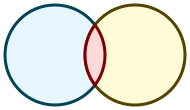
\includegraphics[width=0.5\tw]{example.svg.pdf}

  \caption{\textbf{Example Figure Title --} \normalfont{Descriptive text
      which usually also describes any acronyms used in the figure.}}
  \label{fig-example}

\end{figure}



\lipsum[1-5]


%=========================================================================
% Approach
%=========================================================================

\section{Approach}
\label{sec-approach}

%=========================================================================
% fig-plot-example
%=========================================================================

\begin{figure}[t]

  \includegraphics[width=\cw]{plot-example.py.pdf}

  \caption{\textbf{Example Figure Title --} \normalfont{Descriptive text
      which usually also describes any acronyms used in the plot.}}
  \label{fig-plot-example}

\end{figure}



\lipsum[1-5]


%=========================================================================
% Methodology
%=========================================================================

\section{Methodology}
\label{sec-methodology}

\lipsum[1-5]


%=========================================================================
% Evaluation
%=========================================================================

\section{Evaluation}
\label{sec-evaluation}

\lipsum[1-5]


%=========================================================================
% Related Work
%=========================================================================

\section{Related Work}
\label{sec-related}

\lipsum[1]~\cite{jiang-mamba-dac2018, bukreyev-dcs-tcasi2018,
  kim-lta-micro2014, srinath-xloops-micro2014}

\lipsum[2-3]


%=========================================================================
% Conclustions
%=========================================================================

\section{Conclusions}
\label{sec-conclusions}

\lipsum[1]



%-------------------------------------------------------------------------
% Back Matter
%-------------------------------------------------------------------------

\section*{Acknowledgment}

This work was supported in part by ...

\bibliographystyle{IEEEtran}
\balance
\bibliography{cbatten}

\end{document}

